\begin{figure}[tb]
\begin{center}
    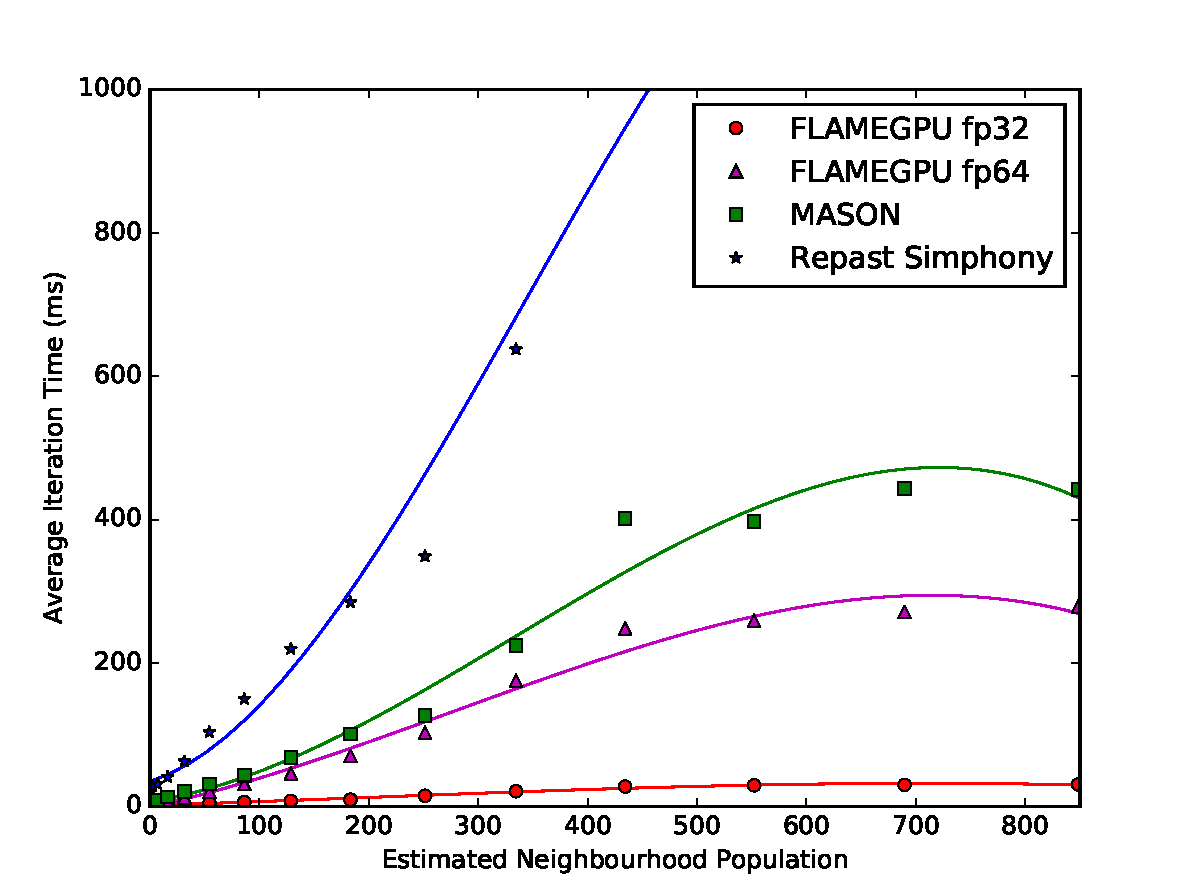
\includegraphics[width=0.7\textwidth]{../resources/problemscale_graph/graph.pdf}
    \caption{\label{fig:graph-agent-pop}The average iteration time of each framework against the agent population.}
\end{center}
\vspace{-1cm}
\end{figure}
\vspace{-0.3cm}
\section{Results\label{sec:results}}
\vspace{-0.4cm}
  Results presented within this section were collected on a single machine running Windows 7 x64 with a Quad core Intel Xeon E3-1230 v3 running at 3.3GHz\footnote{The processor supports hyper-threading, enabling 4 additional concurrent logical threads.}. Additionally the FLAME-GPU framework utilised an Nvidia GeForce GTX 750 Ti \gls{gpu} which has 640 CUDA cores running at 1GHz.
  
  Each of the parameter sets utilised targeted a different performance metric identified in Section \ref{sec:effective-usage}. Results were collected by monitoring the total runtime of 1000 iterations of 3D implementations of the benchmark (executed without visualisation) and are presented as the per iteration mean. Initialisation timings are excluded as the benchmarks focal point is the performance of the nearest neighbours search carried out within each iteration.
  The results in Figure \ref{fig:graph-agent-pop} present the variation in performance as the scale of the problem increases. This is achieved by increasing the parameter $W$, which increases the volume of the environment and hence the agent population. Most apparent from these results is that FLAMEGPU, which utilises \gls{gpu} computation, as opposed to the other frameworks, which utilise a multi-threaded \gls{cpu} approach, consistently outperforms the best multi-core framework by a margin of 2-5 times. This is in line with the expectations of \gls{gpu} accelerated computation\cite{LK*10}. Although MASON and Repast Simphony are both Java based frameworks, MASON's performance trailed that of Repast by around 2-3x. Observation during runtime showed MASON with much lower multi-core utilisation than Repast, which likely explains this disparity. 
  The MASON and Repast results both have a Pearson correlation coefficient (PCC) \cite{PCC} of 0.99. This is indicative of a linear relationship. Similarly FLAMEGPU has a PCC of 0.99 when only agent populations of 150,000 and higher are considered, This suggests that smaller agent populations did not fully utilise the \gls{gpu}.
  % Width: 50,60..300
  % Density: 0.01
  % Interaction Rad: 5.0
  % Attraction Force: 0.00001
  % Repulsion Force: 0.00001
  % Iterations: 1000
  \begin{figure}[tb]
\begin{center}
    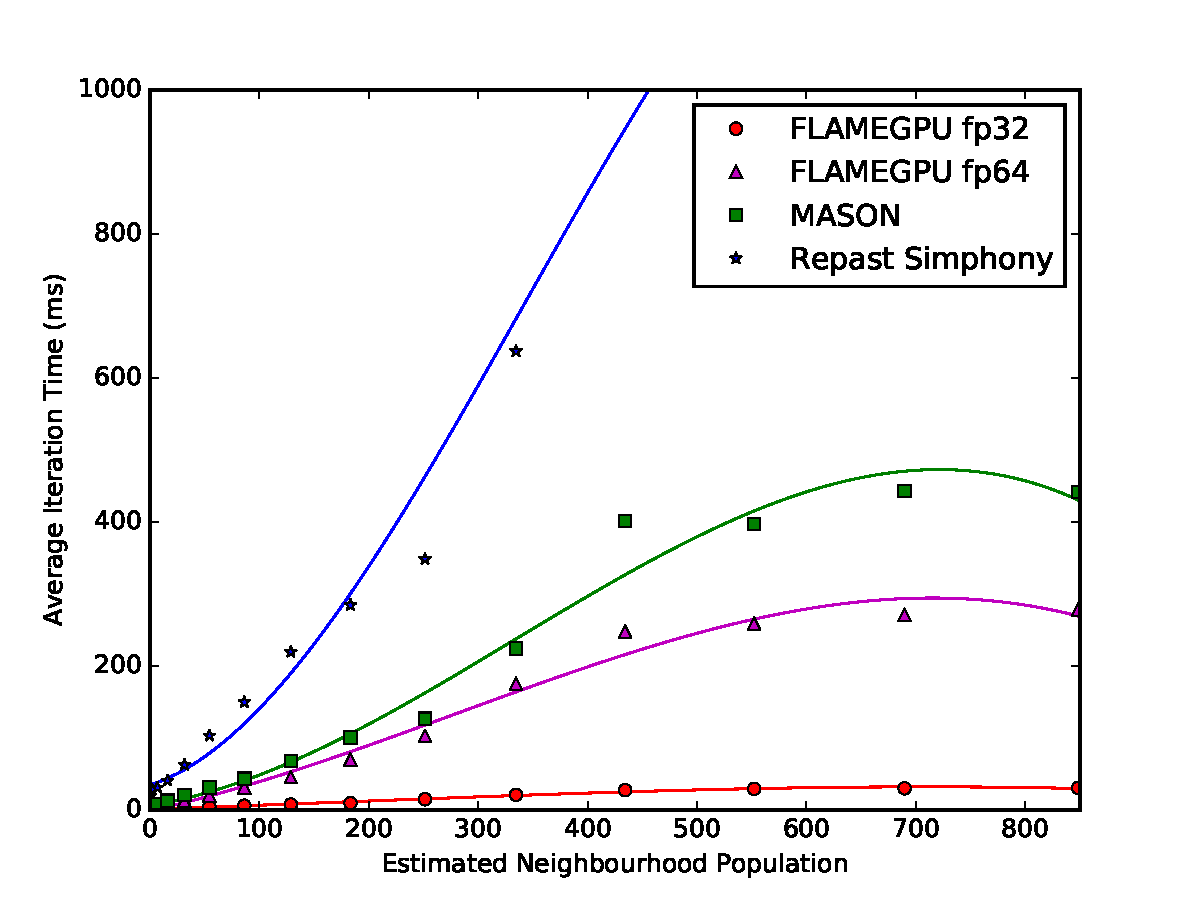
\includegraphics[width=0.7\textwidth]{../resources/neighbourscale_graph/graph.pdf}
    \caption{\label{fig:graph-neighbourhood-pop}The average iteration time of each framework against the estimated neighbourhood population.}
\end{center}
\vspace{-1cm}
\end{figure}
  
  The next parameter set, shown in Figure \ref{fig:graph-neighbourhood-pop}, assessed the performance of each framework in response to increases in the agent populations within each neighbourhood. The purpose of this benchmark set was to assess how each framework performed when agents were presented with a greater number of neighbours to survey. This was achieved by increasing the parameter $r$, hence increasing the volume of each agent's radial neighbourhood. The MASON and Repast Simphony results both have a PCC \cite{PCC} of 0.98. This is indicative of a linear relationship. FLAMEGPU by contrast has a PCC of 0.90, suggesting weaker positive correlation. MASON initially outperformed Repast, however the effect of increased neighbourhood sizes saw Repast perform quicker when neighbourhoods were greater than 6 agents.
  % Width: 100
  % Density: 0.01
  % Interaction Rad: 1,2..15
  % Attraction Force: 0.00001
  % Repulsion Force: 0.00001
  % Iterations: 1000
  The final parameter set assessed variation in performance in response to increased entropy. This is achieved by adjusting the parameters $k_{att}$ and $k_{rep}$, causing the force exerted on the agents to increase, subsequently causing them to move faster.
  The purpose of this benchmark was to assess whether any of the frameworks benefited from reduced numbers of agents transitioning between spatial partitions. The results however showed that performance for each framework remained stable throughout all parameters as expected (See Section \ref{sec:effective-usage}).
  % Width: 50,60..300
  % Density: 0.01
  % Interaction Rad: 5.0
  % Attraction Force: 0.00001
  % Repulsion Force: 0.00001
  % Iterations: 100